
%\renewcommand{\thefigure}{\theenumi.\arabic{figure}}
\begin{figure}[!ht]
\centering
\resizebox{\columnwidth}{!}{%\documentclass{standalone}
%
%\usepackage{tikz,pgf} %and any other packages or tikzlibraries your picture needs
%
%\begin{document}
%\resizebox{\columnwidth}{!}{
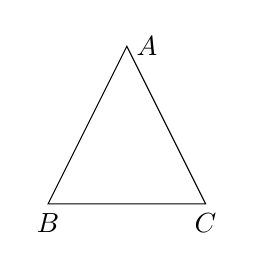
\begin{tikzpicture}
\draw (0,0) node[anchor=north]{$B$}
  -- (1,2) node[anchor=west]{$A$}
  -- (2,0) node[anchor=north]{$C$}
  -- cycle;
\end{tikzpicture}
%}
%\end{document}}
\caption{$\triangle ABC$ and $\triangle PQR$ by Latex-Tikz}
\label{fig:8.1.36_triangle_latex}	
\end{figure}
%
%
%\renewcommand{\thefigure}{\theenumi}
%

\item {\em Construction: }The coordinates of the various points of triangle ABC in Fig. \ref{fig:8.1.36_triangle_latex} are
%\label{}
%
\begin{align}
\vec{B} &= \myvec{0\\0} ,
\label{eq:8.1.36_constr_b}
\\
 \vec{C} &= \myvec{a\\0}, 
\label{eq:8.1.36_constr_c}
\end{align}

$\because \vec{M}$ is the midpoint of $BC$,
\begin{align}
\vec{M}= \frac{\vec{B}+\vec{C}}{2} =\myvec{a/2\\0},
\label{eq:8.1.36_constr_m}
\end{align}
%
$\triangle PQR$ is a horizontal translation of $\triangle ABC$.  Hence, if 
\begin{align}
\vec{Q}= \myvec{q\\0},
\label{eq:8.1.36_constr_q}
\end{align}
\begin{align}
\vec{P}= \vec{A} + \vec{Q}
\\
\vec{R}= \vec{C} + \vec{Q}
\end{align}

%



